\section{Seeding by RF Noise} \label{Seed}

Seeding is important in RNG designs as it is fundamental to the randomness of PRNG. CC2538 suggests in its manual to  use the RF core to generate sample seed, as quote as:(Section 16.2.2 in CC2538 User's Guide\cite{CC2538Manual})
\begin{quote}
For the CC2538, when a random value is required, writing the SOC\_ADC\_RNDL register with random bits from the IF\_ADC in the RF receive path seeds the LFSR.
\end{quote}
and: (Section 23.12 in CC2538 User's Guide\cite{CC2538Manual})
\begin{quote}
Single random bits from either the I or Q channel can be read from the RFRND register.
\end{quote}
In case of Contiki, the driver only used the bits generated in I channel.

For the randomness of this seeding method, the manual\cite{CC2538Manual} reported: (Section 23.12 in CC2538 User's Guide\cite{CC2538Manual})
\begin{quote}
Randomness tests show good results for this module. However, a slight DC component exists. In a simple test where the RFRND.IRND register was read a number of times and the data was grouped into bytes, about 20 million bytes were read. When interpreted as unsigned integers between 0 and 255, the mean value was 127.6518, which indicates that there is a DC component.
...
For the first 20 million individual bits, the probability of a 1 is $P(1) = 0.500602$ and $P(0) = 1 - P(1) = 0.499398$.
\end{quote}

Their test results are shown in \Cref{SeedResult}.

\begin{figure}[!t]
\centering
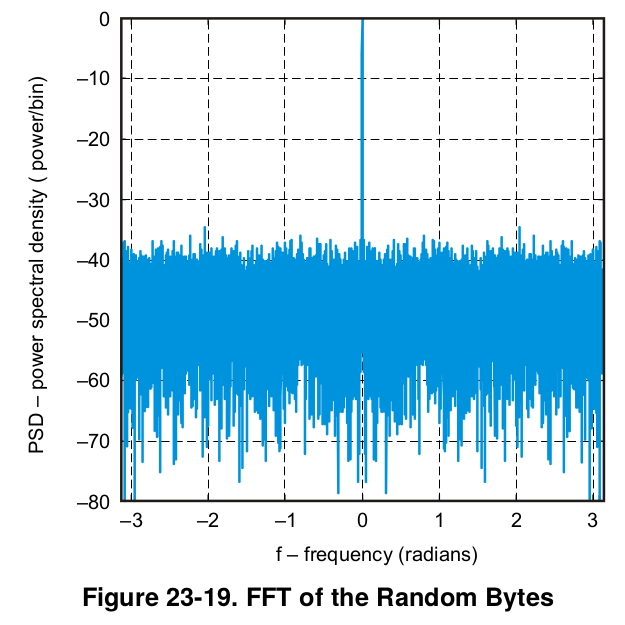
\includegraphics[width=2.5in]{fig/CC2538_Seed1.png}
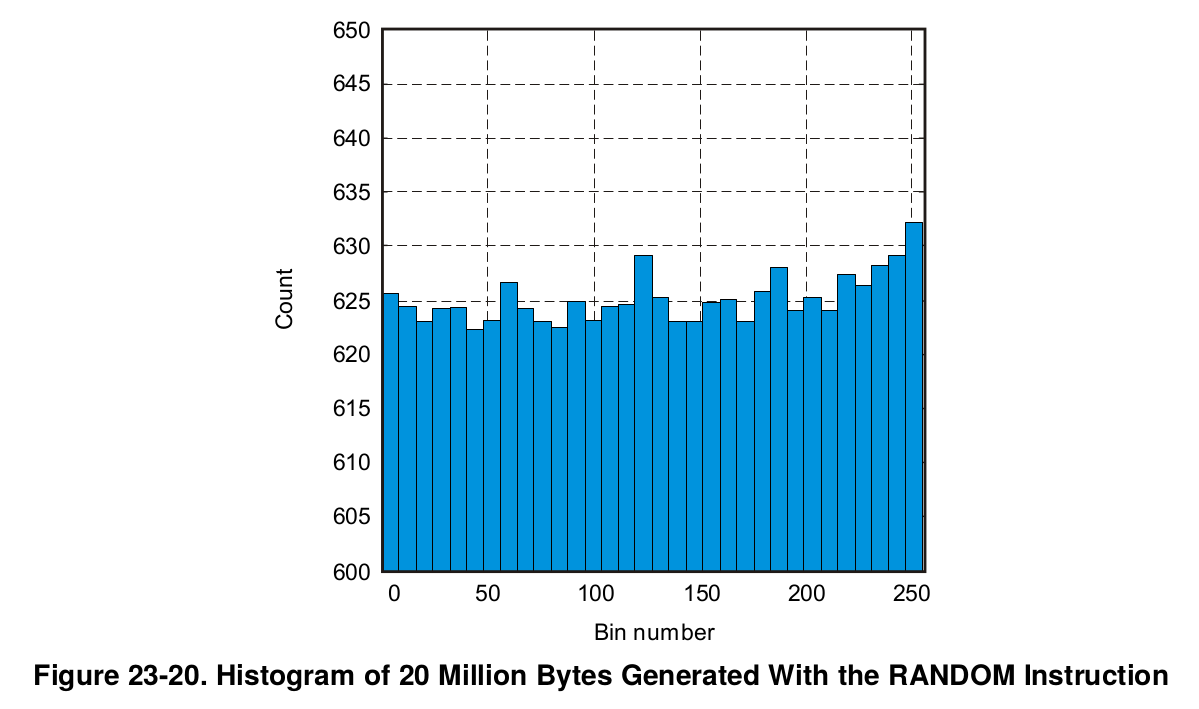
\includegraphics[width=2.5in]{fig/CC2538_Seed2.png}
\caption{RF core seeding result, from CC2538 User's Guide}
\label{SeedResult}
\end{figure}

To further verify the randomness of this seeding method, we applied the NIST Statistical Test Suite\cite{NISTTest} on 13263600 bits sampled by this seeding method using our application in \cite{prngtest}. Since each read to RFRND generates only $1$ bit, we concatenated all bits into one bit stream of length $13263600$. The bits has passed all tests in the NIST test suite, with $P(0) = 0.49995001$ and $P(1) = 0.50004999$. The full report and raw data are applicable at \cite{prngtest}.

Despite the good randomness of the seed, sampling from RF noise remains sceptical from a security perspective as such physical source can be easily tampered remotely by sending signal wave to the device.

The released documents did not explain further details of how the output of IF\_ADC in the receive I/Q channels translated to random bits. We have neither found any open document describes  the RF design of CC2538. 

However, we noticed the same RNG design has been applied on several product in TI's SimpleLink\texttrademark series. Some of them provided better explanation of their design of RF core and RNG which could be a hint to CC2538. In CC2430 user manual\cite{CC2430Manual}, we found a description of the RF core, shown in \Cref{CC2430RF}.

\begin{figure}[!t]
\centering
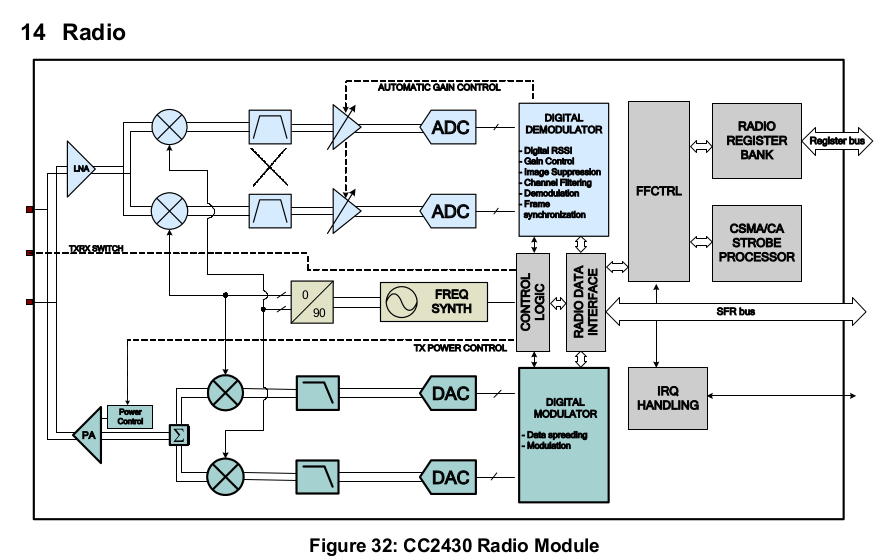
\includegraphics[width=2.5in]{fig/CC2430_Radio.png}
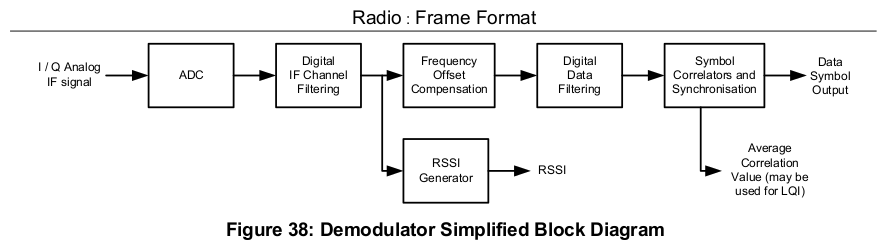
\includegraphics[width=2.5in]{fig/CC2430_Demodulator.png}
\caption{CC2430 RF Design, from CC2430 user manual\cite{CC2430Manual}}
\label{CC2430RF}
\end{figure}

\Cref{CC2430RF} suggests that the input analogue signal to IF\_ADC has went through the following components:
\begin{itemize}
	\item Low Noise Amplifier (LNA) which amplifies the signal.
	\item Mixer which down converts the signal frequency. The Frequency Synthesiser is used as the local oscillator.
	\item Band pass filter which filters out the out of band signals.
	\item The Automatic Gain Control (AGC) circuit which further adjusts the signal strength to the input level of ADC.
\end{itemize}

CC2520 Data Sheet\cite{CC2520Manual} explains the random bit is actually the Least Significant Bit (LSB) from ADC: (Section 24 in \cite{CC2520Manual})
\begin{quote}
Single random bits from either the I or Q channel (configurable) can be output on GPIO pins at a rate of 8MHz. One can also select to xor the I and Q bits before they are output on a GPIO pin. These bits are taken from the least significant bit in the I and/or Q channel after the decimation filter in the demodulator.
\end{quote}

A block diagram is also provided, as shown in \Cref{CC2520RFRND}.
\begin{figure}[!t]
\centering
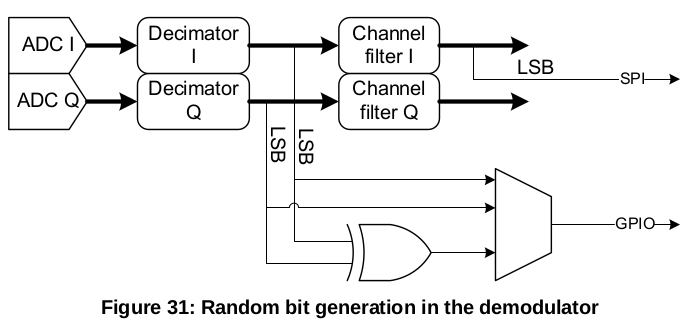
\includegraphics[width=2.5in]{fig/CC2520_RNG.png}
\caption{CC2520 RNG Design, from CC2520 user manual\cite{CC2520Manual}}
\label{CC2520RFRND}
\end{figure}

Interestingly, we noticed that CC2538, CC2520, CC253X and CC2540/41 reported exactly the identical randomness test result in their user manuals (\cite{CC2538Manual} \cite{ CC2520Manual} \cite{CC2530Manual}). This suggests they are very likely to have the same seeding design.

Assuming the same design has been applied to CC2538, it would explained the nice randomness of the seeding method. Denote $V$ as analogue RF signal and $N$ as noise, the analogue input to the ADC $V_{in}$ can be represented as:
\begin{equation}
V_{in} = V + N
\end{equation}

The noise $N$ can be induced by multiple sources in practice, including:
\begin{itemize}
\item Noise produced by the signal source.
\item Environmental noise.
\item Noise induced by the components in the device itself.
\end{itemize}
In practice, manipulating the noise could be difficult.

The random bit $b$ can be represented as:
\begin{equation} \label{RNDOutput}
b = LSB(V_{in}) = LSB(V + N)
\end{equation}
where $LSB() \in \{0,1\}$ represents the operation of taking the LSB of A/D conversion output.

Observing \Cref{RNDOutput}, one thing to be noticed is that any difference in $V_{in}$ larger than the scale of ADC, i.e. the voltage represented by its LSB, could flip $b$. According to CC2538 data sheet\cite{CC2538Datasheet}, the receiver can be sensitive to signals down to $-97dBm$ (typical value with $T_A = 25^{\circ}C$, $V_{DD} = 3V$ and $f_{C} = 2440MHz$). On the other hand, the typical environmental noise in our experimental environment, which is a typical office with multiple noise sources such as  WiFi, smart phones, etc, is about $-92dBm$ which is significantly higher than the receiver sensitivity. We consider the result of the randomness test as an evidence to this sampling method.

\section{Biasing Seed by Radio Jamming}
At a first glance one way to bias the seed is to generate a predictable $V_{in}$. \Cref{RNDOutput} indicates that the random bit $b$ is jointly determined by the signal $V$ and noise $N$. Even though $V$ can be viewed as being controlled by the adversary, manipulating $N$ turns out to be difficult in practice. For instance, noises accumulated by different amplification stages are physically inevitable. Hence fixing $V_{in}$ does not seem to be easily achievable in practice.

Therefore an alternative attempt is to provide the RF with an illegal $V_{in}$. Two methods are considered in our experiments:
\begin{itemize}
	\item Saturation. This method attempts to provide the RF with a strong signal that is above its acceptance level.
	\item Decimation. This method attempts to provide the RF with a weak signal that is beneath its acceptance level.
\end{itemize}

Ideally we expect these illegal inputs will trigger the ADC into a fault state which could potentially result into a predictable output and thus predictable $b$. But in practice, decimation does not seem practical for the same reason that noises induced by the circuits themself is physically inevitable. This made saturation the only viable option.

Meanwhile, the undisclosed circuit design of the device also poses a great difficulty in our experiments as without knowledge of the exact circuit designed it would be difficult to the deduce the most effective signal as well as to predict the outcome. We have only performed black box experiments on OpenMote which is a CC2538 based SoC.

\subsection{Sine wave signal}

\subsection{Sawtooth sine wave signal}

\subsection{Pulse signal}
